\begin{pastexam}[label={px:ntu-111-dsaa-19}]{臺大資工所 111 學年度 第 19 題}
（單選）

(5 points) Consider the following undirected graph $G$. Let $T$ be the minimum spanning tree (MST)
of the graph. Which is INCORRECT?

\begin{center}
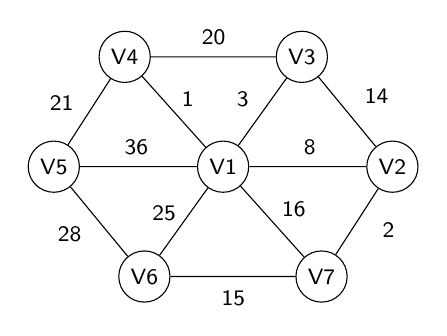
\begin{tikzpicture}[x=1cm,y=-0.9cm,v/.style={circle,draw,inner sep=0pt,minimum size=6.5mm,font=\footnotesize\sffamily},w/.style={font=\footnotesize\sffamily,inner sep=1pt}]
\node[v] (v4) at (1.95,1.05) {V4}; \node[v] (v3) at (4.2,1.05) {V3};
\node[v] (v5) at (1.05,2.6) {V5}; \node[v] (v1) at (3.2,2.6) {V1}; \node[v] (v2) at (5.35,2.6) {V2};
\node[v] (v6) at (2.2,4.15) {V6}; \node[v] (v7) at (4.45,4.15) {V7};
\draw (v4)--(v3) (v3)--(v2) (v2)--(v7) (v7)--(v6) (v6)--(v5) (v5)--(v4)
  (v1)--(v4) (v1)--(v3) (v1)--(v2) (v1)--(v7) (v1)--(v6) (v1)--(v5);
\node[w] at (3.08,0.78) {20}; \node[w] at (1.15,1.7) {21}; \node[w] at (2.75,1.65) {1}; \node[w] at (3.45,1.65) {3};
\node[w] at (5.15,1.6) {14}; \node[w] at (2.1,2.32) {36}; \node[w] at (4.3,2.32) {8}; \node[w] at (2.45,3.25) {25};
\node[w] at (4.1,3.2) {16}; \node[w] at (1.25,3.55) {28}; \node[w] at (5.3,3.5) {2}; \node[w] at (3.33,4.45) {15};
\end{tikzpicture}
\end{center}
\begin{enumerate}[label=(\Alph*)]
\item Edge $(V_1,V_4)$ is in $T$
\item Edge $(V_4,V_5)$ is in $T$
\item Let $w_{4,5}$ be the weight of $(V_4,V_5)$. If we decrease $w_{4,5}$ by 16 (i.e., $w_{4,5}$
becomes 5), then $T$ remains to be the MST of $G$
\item Let $w_{2,3}$ be the weight of $(V_2,V_3)$. If we decrease $w_{2,3}$ by 10 (i.e., $w_{2,3}$
becomes 4), then $T$ remains to be the MST of $G$
\item none of the other choices
\end{enumerate}
\end{pastexam}

\begin{pastsoln}
答案是 (D)。

先求 $T$。 圖有 $7$ 個頂點、$12$ 條邊，權重各不相同，所以最小生成樹只有一棵（資結書定理~24.4）。 用
Kruskal（資結書第~24.2~節），邊依權重由小到大：
\begin{center}
\begin{tabular}{cll}
\toprule
權重 & 邊 & 結果 \\
\midrule
1 & $V_1V_4$ & 加入 \\
2 & $V_2V_7$ & 加入 \\
3 & $V_1V_3$ & 加入 \\
8 & $V_1V_2$ & 加入，$\{V_1, V_2, V_3, V_4, V_7\}$ 連成一塊 \\
14 & $V_2V_3$ & 跳過（$V_2$--$V_1$--$V_3$ 已連通） \\
15 & $V_6V_7$ & 加入 \\
16 & $V_1V_7$ & 跳過 \\
20 & $V_3V_4$ & 跳過 \\
21 & $V_4V_5$ & 加入，共 $6$ 條，完成 \\
\bottomrule
\end{tabular}
\end{center}
$T = \{V_1V_4, V_2V_7, V_1V_3, V_1V_2, V_6V_7, V_4V_5\}$，權重 $1 + 2 + 3 + 8 + 15 + 21 = 50$。
\begin{itemize}
\item (A) 對：$V_1V_4$（權重 $1$）在 $T$ 裡。
\item (B) 對：$V_4V_5$（權重 $21$）在 $T$ 裡。 $V_5$ 的三條邊是 $21$、$28$、$36$，最輕的 $21$ 一定在
最小生成樹裡（切割性質，資結書定理~24.1，切割取 $\{V_5\}$）。
\item (C) 對。 降低一條\textbf{樹邊}的權重，$T$ 仍然是最小生成樹：$T$ 的權重少了 $16$；任何其他生成樹
$T'$ 的權重最多也只少 $16$（含這條邊時），原本 $w(T) \le w(T')$，改完仍是 $w(T) - 16 \le w'(T')$。
重新跑 Kruskal 也一樣：權重 $5$ 的 $V_4V_5$ 排在 $3$ 和 $8$ 之間加入，選出的仍是同樣六條邊。
\item (D) \textbf{錯}。 $V_2V_3$ 不在 $T$ 裡。 把它加進 $T$ 會形成環 $V_2$--$V_1$--$V_3$--$V_2$，環上
的邊權重是 $8$、$3$ 和新的 $4$。 環上最重的是 $V_1V_2$（$8$），由環性質（資結書定理~24.3），它不在
新的最小生成樹裡；把它換成 $V_2V_3$ 得到權重 $50 - 8 + 4 = 46 < 50$ 的生成樹，所以 $T$ 不再是最小
生成樹。
\item (E)：(D) 錯，不選。
\end{itemize}
\end{pastsoln}
